\documentclass[a4paper, 11pt]{article}
\usepackage{geometry}
\geometry{letterpaper, margin=1in}
\usepackage{graphicx}
\graphicspath{ {images/} }

\usepackage{amsmath}
\usepackage{amssymb}  
\usepackage{amsthm}
\usepackage{ulem}

\usepackage{enumitem}


\usepackage{pdfpages} % for including full pdf pages

\usepackage{empheq}

\usepackage{listings}


%format to allow bolded theorems, corollaries, etc...
\newtheorem*{theorem}{Theorem}
\newtheorem*{corollary}{Corollary}
\newtheorem*{lemma}{Lemma}
\newtheorem*{definition}{Definition}
\newtheorem*{Example}{Example} 
\newtheorem*{Remark}{Remark}

% stop typing \mathbb a thousand times 
\newcommand{\R}{\mathbb{R}}
\newcommand{\C}{\mathbb{C}}
\newcommand{\F}{\mathbb{F}}
\newcommand{\E}{\mathbb{E}}
\newcommand{\M}{\mathbb{M}}
\newcommand{\sphere}{\mathbb{S}}

% commands for bra-ket notation
\newcommand{\bra}[1]{\ensuremath{\left\langle#1\right|}}
\newcommand{\ket}[1]{\ensuremath{\left|#1\right\rangle}}
\newcommand{\bracket}[2]{\ensuremath{\left\langle #1 \middle| #2 \right\rangle}}
\newcommand{\matrixel}[3]{\ensuremath{\left\langle #1 \middle| #2 \middle| #3 \right\rangle}}
\newcommand{\expectation}[1]{\ensuremath{\left\langle #1 \right\rangle}}

% vector stuff
\newcommand{\basis}[1]{\hat{\mathbf{e}}_#1}
\newcommand{\unit}[1]{\hat{\boldsymbol{#1}}}
\newcommand{\bvec}[1]{\vec{\boldsymbol{#1}}}
\newcommand{\threevec}[2]{\begin{pmatrix} #1 \\ #2 \end{pmatrix}}

% change margins for solution
\newenvironment{solution}{%
	\begin{list}{}{%
			\setlength{\topsep}{0pt}%
			\setlength{\leftmargin}{0.5cm}%
			\setlength{\rightmargin}{0.5cm}%
			\setlength{\listparindent}{\parindent}%
			\setlength{\itemindent}{\parindent}%
			\setlength{\parsep}{\parskip}%
		}%
		\item[]}{\end{list}}




\begin{document}
\noindent
\large\textbf{Homework 1} \hfill \textbf{John Waczak} \\
\normalsize MTH 437 \hfill  Date: \today \\
Dr. Tevian Dray %\hfill worked w/ Ryan Tollefsen
\par\noindent\rule{\textwidth}{0.4pt} \\\\



\begin{enumerate}[leftmargin=0em, label=\textbf{\arabic*}]
  \item \textbf{VECTORS IN MINKOWSKI SPACE}\\
    Show that a timelike vector cannot be orthogonal to a null vector or to another timelike
    vector. Show that two null vectors are orthogonal if and only if they are parallel. (Assume
    these vectors are nonzero.)

    \textit{Try to do this in 4 spacetime dimensions rather than 2. A convenient
    notation is to view a 4-vector $\mathbf{u}$ as consisting of a timelike
    component $u^t$ and spacelike components making up an ordinary 3-vector
    $\bvec{u}$; one often writes}
    \begin{equation}
      \mathbf{u} = \threevec{u^t}{\bvec{u}}
    \end{equation}

    \begin{solution}
      Let $\mathbf{u}\in\M^4$ with $|\mathbf{u}|>0$ be a timelike vector representing the
      motion of some object; that is, $(u^t)^2>|\bvec{u}|^2$. Assume without loss of
      generality that $\bvec{u} = |\bvec{u}|\basis{i}$. We can always choose an
      appropriate hyperbolic rotation by some angle $\alpha$ so that in the object's
      rest frame, $\mathbf{u}$ is given by
      \begin{equation}
        \mathbf{u} = \threevec{u^t}{\bvec{0}}
      \end{equation}
      Now consider a second vector $\mathbf{v}$ with $|\mathbf{v}|>0$. In
      general, if $\mathbf{v}$ is timelike we may write
      \begin{equation}
        \mathbf{v} = \pm|\mathbf{v}|\threevec{\cosh\beta}{\sinh\beta\unit{v}}
      \end{equation}
      in order to make the timelike quality explicit.\\

      Taking the inner product yields
      \begin{equation}
        \mathbf{u}\cdot\mathbf{v} = \mp|v|\cosh\beta u^t \neq 0
      \end{equation}
      because $\cosh\beta>0$ $\forall \beta$. \\

      If instead $\mathbf{v}$ is a null vector, then it may be written in as
      \begin{equation}
        \mathbf{v} = a\threevec{1}{\unit{v}}
      \end{equation}
      for any $a\neq 0$. The inner product with $\mathbf{u}$ yields
      \begin{equation}
        \mathbf{u}\cdot\mathbf{v} = au^t \neq 0 
      \end{equation}
      Therefore, we conclude that a timelike vector in $\M^4$ cannot be
      orthogonal to a timelike vector or a null vector.\\

      For the second part of the question, let $\mathbf{u},\mathbf{v}\in \M^4$
      be null vectors. That is,
      \begin{equation}
        \mathbf{u}=a\threevec{1}{\unit{u}} \qquad \mathbf{v}= b\threevec{1}{\unit{v}}
      \end{equation}
      Let's do the forward direction $(\rightarrow)$ first. Assume that
      $\mathbf{u}\parallel\mathbf{v}$. In other words $\unit{v}=\unit{u}$. Then
      taking the inner product yields
      \begin{equation}
        \mathbf{u}\cdot\mathbf{v} = ab(\unit{u}\cdot\unit{u}-1) = 0 
      \end{equation}
     Therefore, $\mathbf{u}\parallel\mathbf{v}$  implies that
     $\mathbf{u}\cdot\mathbf{v}=0$.\\

     For the reverse direction $(\leftarrow)$, assume that
     $\mathbf{u}\cdot\mathbf{v}=0$. Then the inner product gives
     \begin{align}
       0 &= ab(\unit{u}\cdot\unit{v}-1) \\
       \Rightarrow &\unit{u}\cdot\unit{v} = 1 
     \end{align}
     which is precisely the condition for $\mathbf{u}\parallel\mathbf{v}$.
     Therefore we conclude that two null vectors are orthogonal if and only if
     they are parallel. 
        
      
    \end{solution}
    

  \item \textbf{EARTH DISTANCE}\\
    Corvallis is located at approximately $(44.55^\circ N, 123.25^\circ W)$,
    that is, $44.55^\circ$ north of the equator (latitude), and $123.25^\circ$
    west of the prime meridian (longitude). Tangent is located at approximately
    $(44.55^\circ N, 123.1^\circ W)$, and Eugene is at approximately
    $(44.05^\circ N, 123.1^\circ W)$. Gresham, OR, is located at approximately
    $(45.50^\circ N,122.4 W)$, Millbrae, CA, is located at approximately
    $(37.60^\circ N,122.4^\circ W)$, and Richmond, VA, is at approximately
    $(37.60^\circ N, 77.50^\circ W)$. \\

    \textit{Assume that the Earth is a perfect sphere with radius $r=3959$ mi
      with line element}
    \begin{equation}
      ds^2 = r^2(d\theta^2 + \sin^2\theta d\phi^2)
    \end{equation}
    
    
    \begin{enumerate}[leftmargin=2em, label=(\textbf{\alph*})]
    \item Approximate the following distances using the Pythagorean Theorem:\\
      Corvallis to Tangent; Tangent to Eugene; Corvallis to Eugene.\\
      \begin{solution}
        \begin{figure}[!hbt]
          \centering
          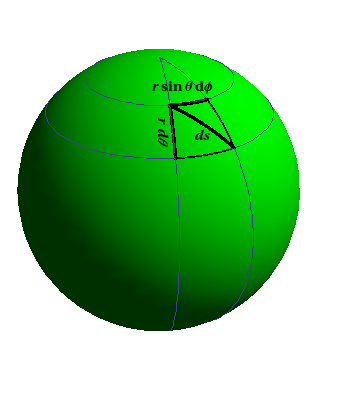
\includegraphics[width=0.4\columnwidth]{sphere_triangle}
          \caption{An infinitesimal triangle on the surface of the sphere. Image
            taken from [Dray 2015].}
          \label{fig:sphere}
        \end{figure}

        Figure \ref{fig:sphere} shows a sphere with an infinitesimal triangle
        whose side lengths are given by the and hypotenuse are given by the
        equation (11) for the line element. In order to approximate these
        distances, we can find $\Delta \theta$ and $\Delta \phi$ from the given
        information and then pick a value for $\theta$ to use. \textbf{NOTE} the
        latitude is measured in degrees north of the equator but we must instead
        use the compliment for $\theta$ because the spherical inclination is
        measured from the pole. This is not a problem for $\Delta \theta$
        and $\Delta \phi$  as all that matters for these is the difference in
        angle.\\

        We will choose the greater of the inclination angles to use as $\theta$.
        Thus, we have the following
        \begin{align}
          \Delta \theta_{\text{corv, tang}} &= 0^\circ = 0 \quad \text{rad}\\
          \Delta \phi_{\text{corv, tang}} &= 123.25-123.1 = 0.15^\circ \approx 0.0026 \quad \text{rad} \\
          \theta &= 90^\circ-44.55^\circ  = 44.45^\circ \approx 0.775 \quad \text{rad} \\
          \Delta s_{\text{corv, tang}} &= \sqrt{3959^2(0^2+\sin^2(0.775)0.0026^2)} = 7.2 \quad \text{mi} 
        \end{align}

        \begin{align}
          \Delta \theta_{\text{tang, eug}} &= 44.55^\circ-44.05^\circ \approx 0.0087 \quad \text{rad}\\
          \Delta \phi_{\text{tang, eug}} &= 123.1-123.1 \approx 0\quad \text{rad} \\
          \theta &= 90^\circ-44.05^\circ  = 45.95^\circ \approx 0.802 \quad \text{rad} \\
          \Delta s_{\text{tang, eug}} &= \sqrt{3959^2(0.0087^2+\sin^2(0.802)0^2)} = 34.44 \quad \text{mi} 
        \end{align}
 
        \begin{align}
          \Delta \theta_{\text{corv, eug}} &= 44.55^\circ-44.05^\circ \approx 0.0087 \quad \text{rad}\\
          \Delta \phi_{\text{corv, eug}} &= 123.25-123.1 \approx 0.0026\quad \text{rad} \\
          \theta &= 90^\circ-44.05^\circ  = 45.95^\circ \approx 0.802 \quad \text{rad} \\
          \Delta s_{\text{corv, eug}} &= \sqrt{3959^2(0.0087^2+\sin^2(0.802)0.0026^2)} = 35.2 \quad \text{mi} 
        \end{align}
      \end{solution}
      
    \item
      How good are your approximations?

      \begin{solution}
        After a google search, it looks like the correct distances are 8.46 mi,
        34.05 mi, and 37.06 mi... so not too bad!
      \end{solution}

    \item
      Approximate the following distances using the Pythagorean Theorem:\\
      Gresham to Millbrae; Millbrae to Richmond; Gresham to Richmond.

      \begin{solution}
         
        \begin{align}
          \Delta \theta_{\text{gresh, mill}} &= 44.50^\circ-37.60^\circ \approx 0.1204 \quad \text{rad}\\
          \Delta \phi_{\text{corv, eug}} &= 122.4^\circ-122.4^\circ = 0 \quad \text{rad} \\
          \theta &= 90^\circ-37.60^\circ  = 45.95^\circ \approx 0.9146 \quad \text{rad} \\
          \Delta s_{\text{corv, eug}} &= \sqrt{3959^2(0.1204^2+\sin^2(0)0.9146^2)} = 476 \quad \text{mi} 
        \end{align}
       
        \begin{align}
          \Delta \theta_{\text{mill, rich}} &= 37.60^\circ-37.60^\circ = 0 \quad \text{rad}\\
          \Delta \phi_{\text{mill, rich}} &= 122.4^\circ-77.5^\circ = 0.7837 \quad \text{rad} \\
          \theta &= 90^\circ-37.60^\circ  = 45.95^\circ \approx 0.9146 \quad \text{rad} \\
          \Delta s_{\text{mill, rich}} &= \sqrt{3959^2(0^2+\sin^2(0.7837)0.9146^2)} = 2556 \quad \text{mi} 
        \end{align}
 
        \begin{align}
          \Delta \theta_{\text{gresh, rich}} &= 44.5^\circ-37.60^\circ = 0.1204 \quad \text{rad}\\
          \Delta \phi_{\text{gresh, rich}} &= 122.4^\circ-77.5^\circ = 0.7837 \quad \text{rad} \\
          \theta &= 90^\circ-37.60^\circ  = 45.95^\circ \approx 0.9146 \quad \text{rad} \\
          \Delta s_{\text{gresh, rich}} &= \sqrt{3959^2(0.1204^2+\sin^2(0.7837)0.9146^2)} = 2600 \quad \text{mi} 
        \end{align}
      \end{solution}
      
      \item
        How good are your approximations \\

        \begin{solution}
          The correct distances are 545 mi, 2437 mi, and 2359 mi. Again, this is
          pretty impressive for not even integrating. I think if we wanted to be
          exact we would need to parametrize the great circle between the given
          cities and then integrate.
        \end{solution}
    \end{enumerate}
  \end{enumerate}
\end{document}






























